\documentclass[11pt]{article}

\usepackage[margin=1.05in]{geometry}
\usepackage{amsmath, amssymb, amsthm}
\usepackage{graphicx}
\usepackage{booktabs}
\usepackage{microtype}
\usepackage{xcolor}
\usepackage[colorlinks=true, linkcolor=blue!50!black, citecolor=blue!50!black,
            urlcolor=blue!50!black]{hyperref}
\usepackage[numbers, sort&compress]{natbib}

\graphicspath{{figures/}}

\newcommand{\rr}{\mathbf{r}}
\newcommand{\dd}{\mathrm{d}}

\title{Mobility, Algorithms, and Attention:\\
A Stochastic Adaptive Multiplex Model of Opinion Dynamics\\
with Brownian Agents}

\author{Ruben Araujo}
\date{August 2026}

\begin{document}

\maketitle

\begin{abstract}
We introduce a continuous-time model of opinion dynamics in which agents
diffuse through physical space by Brownian motion while simultaneously
interacting through an adaptive, algorithmically curated digital network.
Opinions evolve under bounded-confidence attraction in the physical layer and
under an engagement-weighted influence term in the digital layer, whose
topology coevolves with the opinions through a platform recommendation
kernel. The model incorporates a finite attention budget that forces digital
interaction to displace physical interaction, an
assimilation--indifference--repulsion influence function, and heavy-tailed
influence heterogeneity. Numerical simulations across the four nested levels
of the model yield four main results. (i) Physical mobility controls how many
opinion clusters survive: the number of coexisting clusters decays with the
diffusion coefficient $D$, with the crossover set by the competition between
the local convergence time and the diffusive neighbourhood-renewal time.
(ii) Under opinion-independent (Brownian) mobility, geography never becomes a
predictor of opinion: spatial--opinion correlations remain at noise level for
all $D$, because opposite-minded agents interleave in space instead of
segregating. Ideological structure therefore lives in the network of
interactions, not on the map. (iii) A modest amount of opinion-neutral
long-range digital exposure is enough to melt the locally frozen state and
recover the well-mixed mean-field cluster structure, but an adaptive
similarity-driven recommendation algorithm reverses this effect: as
algorithmic homophily increases, the digital layer reorganises into
ideologically homogeneous, spatially delocalised echo chambers with
near-perfect opinion assortativity and vanishing visible disagreement.
(iv) Once influence includes a repulsive response to strongly opposed views,
every platform design radicalises the population, and the ranking inverts:
the opinion-neutral platform---the consensus machine of the pure
bounded-confidence world---produces the fastest and most extreme
polarization, because uncurated exposure maximises contact with
repulsion-triggering content, while algorithmic homophily, by hiding
disagreement, paradoxically dampens extremism. A phase diagram in the
mobility--digital-attention plane $(D,\lambda)$ locates the consensus,
fragmentation, and polarization regimes.
\end{abstract}

\section{Introduction}
\label{sec:intro}

Continuous-opinion models with bounded confidence, introduced by
\citet{deffuant2000} and \citet{hegselmann2002}, describe populations of
agents who average their opinions only with peers whose views are already
sufficiently close. Despite their simplicity, these models produce the three
canonical outcomes of social influence---consensus, polarization, and
fragmentation---and have become a standard laboratory for studying collective
opinion formation \citep{lorenz2007, castellano2009, bernardo2024}.

Two ingredients of real societies are, however, usually absent from this
laboratory. First, people move. Physical encounters are structured by
geography, and geography changes as individuals commute, migrate, and mix;
the consequences of mobility for bounded-confidence dynamics have only
recently begun to be explored systematically \citep{alraddadi2024}. Second,
people increasingly interact through platforms whose connection topology is
not given but \emph{manufactured}: recommendation algorithms decide who sees
whom, they do so as a function of the very opinions they help shape, and the
resulting feedback between opinions and network structure is a coevolutionary
dynamic in its own right \citep{holme2006, sirbu2019, santos2021,
dearruda2022}. Empirically motivated modelling of echo chambers points to the
same loop of homophilic exposure and reinforcing influence
\citep{baumann2020}, while multiplex formulations show that the coexistence
of several interaction layers can qualitatively change consensus thresholds
\citep{antonopoulos2018}.

This paper combines these ingredients in a single stochastic model, built in
four nested levels so that each mechanism can be switched on and its marginal
effect isolated:

\begin{enumerate}
  \item \textbf{Level 1.} Agents perform Brownian motion in a
  two-dimensional periodic domain and interact through a short-range spatial
  kernel with bounded confidence.
  \item \textbf{Level 2.} A static, opinion-neutral digital layer of
  long-range links is added, sharing a finite attention budget with the
  physical layer.
  \item \textbf{Level 3.} The digital layer becomes adaptive: a
  recommendation kernel rewires attention slots towards ideologically
  similar sources, with an algorithmic-homophily parameter $\gamma$.
  \item \textbf{Level 4.} The platform is generalised to an arbitrary
  engagement function (similarity-driven, neutral, or controversy-driven),
  the influence function acquires an
  assimilation--indifference--repulsion structure
  \citep{kurmyshev2011, tang2025}, and influence strengths become
  heavy-tailed, allowing influencer-like agents; stubborn ``zealot'' agents
  \citep{tian2018} are supported as special nodes.
\end{enumerate}

The Brownian formulation makes the physical layer a genuine
statistical-physics object: the box size $L$ and the diffusion coefficient
$D$ define a spatial mixing time $\tau_{\mathrm{mix}} \sim L^2/D$, which
competes with the opinion convergence time $\tau_{\mathrm{op}} \sim
\alpha^{-1}$. Our central question is how this competition interacts with
the digital layer: \emph{can strong digital connectivity destroy the
geographical structure of opinion while simultaneously increasing
ideological polarization?}

Our simulations answer with a refinement that we did not anticipate when
formulating the model. Mobility does control the surviving number of opinion
clusters, as expected. But under opinion-independent mobility the
geographical structure of opinion that digital media could ``destroy'' never
forms in the first place: spatially close agents converge with their
compatible neighbours, yet incompatible agents remain interleaved at the
same locations, so position and opinion stay uncorrelated at every mobility.
Geographic opinion structure, in this model class, requires
opinion--position coupling (homophilic migration or segregation), not mere
locality of interaction. What the digital layer does control---strongly---is
the \emph{network} structure of opinion: adaptive recommendation produces
near-perfectly assortative, spatially delocalised ideological communities.
A second surprise appears when influence can be repulsive: cross-cutting
exposure of any kind then becomes the engine of radicalisation, and the
platform designs reorder, with the neutral, uncurated platform driving the
population to the extremes faster than either curated design.

\section{Model}
\label{sec:model}

\subsection{State variables}

Each of $N$ agents carries a position $\rr_i(t) \in [0,L)^2$ with periodic
boundary conditions and an opinion $x_i(t) \in [-1,1]$. Agent $i$ may also
carry an influence strength $s_i$ and a stubbornness flag. The digital layer
is a directed graph $A_{ij}(t) \in \{0,1\}$, where $A_{ij}=1$ means that the
platform currently shows content by agent $j$ to agent $i$. Each agent has a
fixed number $k$ of \emph{attention slots}, so that $\sum_j A_{ij} = k$ for
all $i$ and all $t$: attention is conserved, and new digital connections can
only be acquired by dropping old ones.

\subsection{Dynamics}

Positions follow independent Brownian motions,
\begin{equation}
  \dd\rr_i = \sqrt{2D}\,\dd\mathbf{W}_i(t),
  \label{eq:motion}
\end{equation}
with diffusion coefficient $D$. Opinions obey the It\^o equation
\begin{equation}
  \dd x_i =
  \alpha_i \,
  \frac{\sum_j K(r_{ij})\, B_\epsilon(x_j - x_i)\,(x_j - x_i)}
       {\sum_j K(r_{ij})\, B_\epsilon(x_j - x_i)} \,\dd t
  \;+\;
  \beta_i \,
  \frac{\sum_j A_{ij}\, s_j\, F(x_i, x_j)}
       {\sum_j A_{ij}\, s_j} \,\dd t
  \;+\;
  \sigma_x\, \dd B_i(t),
  \label{eq:opinion}
\end{equation}
clipped to $[-1,1]$, where $r_{ij}$ is the minimum-image distance between
agents $i$ and $j$. The physical interaction kernel is a truncated Gaussian,
\begin{equation}
  K(r) = e^{-r^2 / 2\ell^2}\, \mathbf{1}(r < 3\ell),
  \label{eq:kernel}
\end{equation}
and $B_\epsilon(\Delta) = \mathbf{1}(|\Delta| < \epsilon)$ implements bounded
confidence. The truncation in Eq.~\eqref{eq:kernel} is not cosmetic: because
the drift is normalised, an untruncated Gaussian would let an agent with no
nearby compatible peers average with the entire population at $O(1)$ rate
through the exponential tail, making spatial isolation impossible and
silently removing the mobility scale from the problem.

The influence function in the digital term has the
assimilation--indifference--repulsion form
\begin{equation}
  F(x_i, x_j) =
  \begin{cases}
    x_j - x_i, & |x_j - x_i| < \epsilon_1, \\
    0, & \epsilon_1 \le |x_j - x_i| < \epsilon_2, \\
    -\eta\,(x_j - x_i), & |x_j - x_i| \ge \epsilon_2,
  \end{cases}
  \label{eq:influence}
\end{equation}
with the repulsive branch ($\eta > 0$) active only at Level~4; at Levels
2--3, $F$ reduces to plain bounded confidence with threshold
$\epsilon_1 = \epsilon$. Empirical support for repulsive (``negative'')
influence is discussed by \citet{tang2025}.

\subsection{Attention budget}

The rates in Eq.~\eqref{eq:opinion} satisfy
\begin{equation}
  \alpha_i = \alpha_{\mathrm{tot}}\,(1 - \lambda),
  \qquad
  \beta_i = \alpha_{\mathrm{tot}}\,\lambda,
  \qquad \lambda \in [0,1],
  \label{eq:attention}
\end{equation}
so the digital attention share $\lambda$ measures how much of a finite
information-processing capacity is devoted to the platform. Increasing
digital exposure therefore \emph{displaces} physical influence rather than
adding to it, together with the hard slot constraint $\sum_j A_{ij} = k$.

\subsection{The platform: engagement-driven rewiring}

The digital graph coevolves with the opinions. In each interval $\dd t$,
agent $i$ replaces one uniformly chosen attention slot with probability
$\rho\,\dd t$; the platform selects the replacement source $j$ with
probability
\begin{equation}
  P(i \to j) \;\propto\; E\!\left(|x_i - x_j|\right)\, s_j,
  \label{eq:rewire}
\end{equation}
where $E$ is the platform's \emph{engagement kernel}. We compare three
platform designs:
\begin{equation}
  E_{\mathrm{sim}}(\Delta) = e^{-\gamma \Delta},
  \qquad
  E_{\mathrm{neu}}(\Delta) = 1,
  \qquad
  E_{\mathrm{con}}(\Delta) = e^{-(\Delta - \delta)^2 / 2 s^2}.
  \label{eq:engagement}
\end{equation}
The similarity-driven kernel models algorithmic homophily with strength
$\gamma$ \citep{sirbu2019, santos2021}; the neutral kernel is an
opinion-blind baseline; the controversy-driven kernel encodes a platform
that maximises engagement by showing users content at a preferred
ideological distance $\delta$---content different enough to provoke a
reaction, a mechanism conceptually close to the post-distribution algorithms
of \citet{dearruda2022}.

\subsection{Influence heterogeneity and zealots}

At Level 4, influence strengths are drawn from a shifted Pareto distribution
with tail exponent $\kappa$, normalised to unit mean, so a small number of
agents ("influencers") dominate the recommendation distribution in
Eq.~\eqref{eq:rewire} and the digital drift in Eq.~\eqref{eq:opinion}.
Optionally, a subset of agents can be declared stubborn ($\dd x_i = 0$),
representing institutional actors or media sources \citep{tian2018}.

\subsection{Observables}

We measure: the polarization $P = \operatorname{Var}(x)$; the number of
opinion clusters $n_c$ (groups of at least two agents separated by gaps
larger than $0.05$ in sorted opinion space); a categorical state
(consensus: $n_c \le 1$ or $P < 10^{-2}$; polarization: $n_c = 2$;
fragmentation: $n_c \ge 3$); the spatial--opinion correlation, quantified
both by Moran's~$I$ with Gaussian weights and by the \emph{local agreement
gap} $\Pr(|x_i - x_j| < \epsilon \mid r_{ij} < 3\ell) - \Pr(|x_i - x_j| <
\epsilon)$; the opinion assortativity $\rho$ of the digital graph (Pearson
correlation of endpoint opinions across directed edges); the modularity $Q$
of the digital graph with respect to the partition induced by opinion
clusters; and the mean local disagreement $\langle |x_i - \bar{x}_{\partial
i}| \rangle$ between an agent and the average opinion it is shown.

\subsection{Numerical integration}

Equations \eqref{eq:motion}--\eqref{eq:opinion} are integrated by the
Euler--Maruyama scheme. Unless stated otherwise, $N = 200$, $L = 1$,
$\dd t = 0.02$, $\alpha_{\mathrm{tot}} = 1$, $\epsilon = 0.3$,
$\ell = 0.02$, $k = 10$, $\rho = 5$, and runs last $T = 60$ time units
($T = 80$ at Level 4); statistics are averaged over $6$--$8$ independent
realisations ($3$ for the phase diagram). With $\ell = 0.02$ the mean
physical contact degree is $N\pi(3\ell)^2 \approx 2.3$, below the
percolation threshold of the random geometric graph, so the instantaneous
physical contact network is spatially fragmented and locality is meaningful.
The complete implementation is available in the accompanying repository.

\section{Results}
\label{sec:results}

\subsection{Level 1: mobility sets the number of surviving clusters}
\label{sec:level1}

\begin{figure}[t]
  \centering
  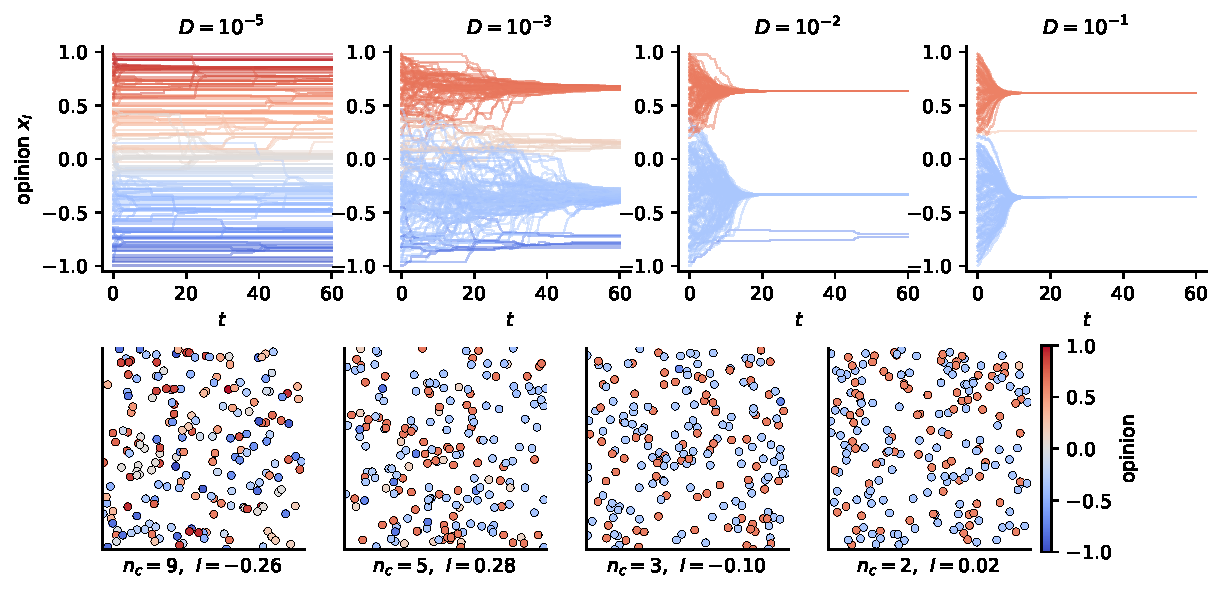
\includegraphics[width=\linewidth]{fig1_mobility.pdf}
  \caption{Purely physical dynamics (Level 1). Top: opinion trajectories
  $x_i(t)$ for increasing diffusion coefficient $D$; colours encode final
  opinions. Bottom: final spatial configurations; markers are agents
  coloured by opinion. Panel captions report the cluster count $n_c$ and
  Moran's $I$. Low mobility freezes many coexisting clusters; high mobility
  approaches the mean-field bounded-confidence outcome. Note the absence of
  spatial colour domains at any $D$.}
  \label{fig:mobility}
\end{figure}

\begin{figure}[t]
  \centering
  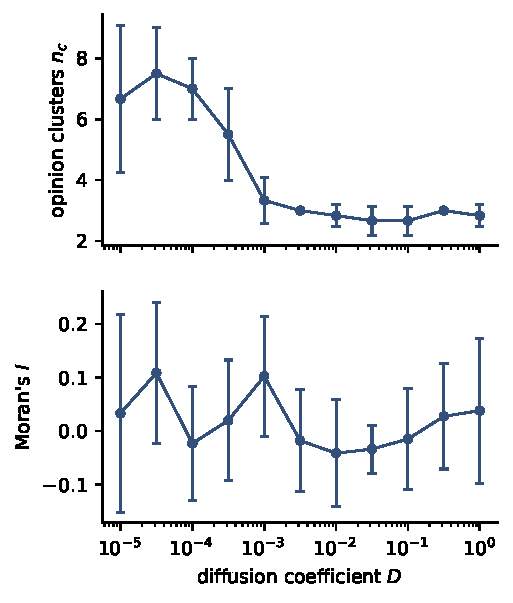
\includegraphics[width=0.85\linewidth]{fig1b_mobility_sweep.pdf}
  \caption{Level-1 sweep over the diffusion coefficient. Left: mean number
  of surviving opinion clusters. Right: Moran's $I$ between opinion and
  position (mean $\pm$ s.d.\ over 6 realisations). Mobility interpolates
  between local fragmentation and mean-field behaviour, while the
  spatial--opinion correlation stays at noise level throughout.}
  \label{fig:mobilitysweep}
\end{figure}

Figures \ref{fig:mobility} and \ref{fig:mobilitysweep} summarise the purely
physical model. The relevant comparison is between the local convergence
time $\tau_{\mathrm{op}} \sim \alpha_{\mathrm{tot}}^{-1}$ and the time
$\tau_\ell \sim \ell^2/D$ over which diffusion renews an agent's
neighbourhood. For $D \lesssim 10^{-4}$ ($\tau_\ell \gg \tau_{\mathrm{op}}$),
compatible agents converge within their frozen local components and the
population fragments into many coexisting clusters ($n_c \approx 5$--$9$).
As $D$ grows, neighbourhood renewal lets clusters within the confidence
bound find each other and merge, and for $D \gtrsim 10^{-2}$ the system
reproduces the well-mixed bounded-confidence outcome ($n_c \approx 2$--$3$
for $\epsilon = 0.3$) \citep{deffuant2000, lorenz2007}. This mobility-driven
fragmentation-to-consensus crossover is consistent with the mobile-agent
simulations of \citet{alraddadi2024}.

The second panel of Fig.~\ref{fig:mobilitysweep} contains the negative
result announced in the Introduction. Moran's $I$---and, equivalently, the
local agreement gap (not shown; it remains below $0.05$ at all
mobilities)---never departs from noise level, \emph{even in the frozen
regime where interactions are strictly local}. The reason is structural:
Brownian positions are opinion-independent, so agents that disagree simply
coexist at the same locations, interacting with disjoint compatible subsets.
Locality controls \emph{how many} opinions survive, but without
opinion-dependent motion (homophilic relocation, avoidance, segregation) it
cannot make geography informative about \emph{which} opinion an agent holds.
Claims that low mobility alone produces geographic echo chambers therefore
need qualification: some coupling between opinion and position is a
necessary ingredient, not a redundant detail.

\subsection{Level 2: opinion-neutral long-range links melt the frozen state}
\label{sec:level2}

\begin{figure}[t]
  \centering
  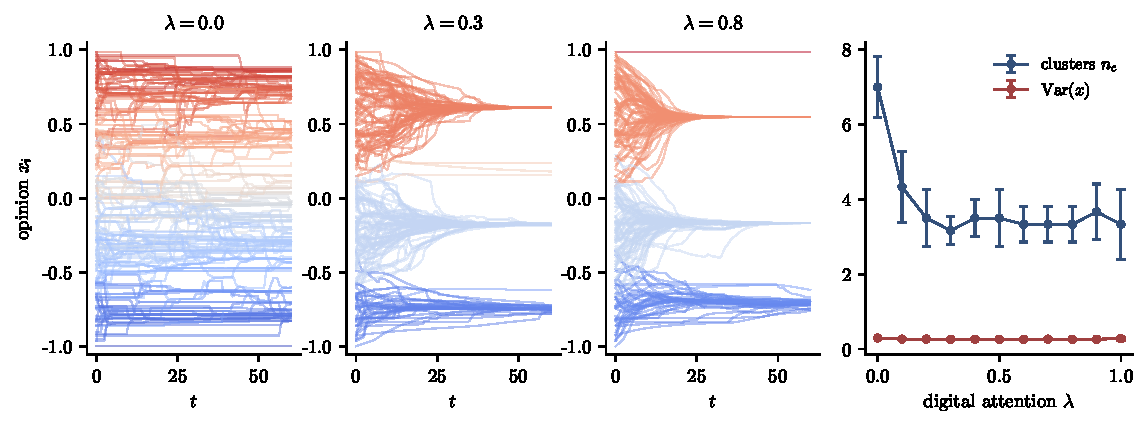
\includegraphics[width=\linewidth]{fig2_static_digital.pdf}
  \caption{Level 2: static random digital layer at low mobility
  ($D = 10^{-4}$). Left three panels: opinion trajectories for increasing
  digital attention share $\lambda$. Right: cluster count and polarization
  versus $\lambda$ (mean $\pm$ s.d.).}
  \label{fig:static}
\end{figure}

Level 2 adds a static, uniformly random directed digital graph ($k = 10$
sources per agent) at low mobility, where the purely physical dynamics
fragments into $n_c \approx 7$ clusters. Figure~\ref{fig:static} shows the
effect of shifting attention to this opinion-neutral layer. Because digital
sources are sampled uniformly, each agent is exposed to the full global
opinion distribution; digital neighbourhoods overlap globally, and a modest
attention share ($\lambda \approx 0.2$) already suffices to merge the
locally frozen clusters into the mean-field cluster set of the well-mixed
bounded-confidence dynamics ($n_c \approx 3$ at $\epsilon = 0.3$), beyond
which additional digital attention changes nothing. Opinion-blind long-range
exposure thus acts exactly like infinite-range mobility: it removes the
excess fragmentation caused by locality---though full consensus would
require a larger confidence bound, as in the classical model
\citep{deffuant2000, antonopoulos2018}. This makes the contrast with the
next level sharp: the consequences of connectivity depend entirely on how
it is curated.

\subsection{Level 3: algorithmic homophily builds delocalised echo chambers}
\label{sec:level3}

\begin{figure}[t]
  \centering
  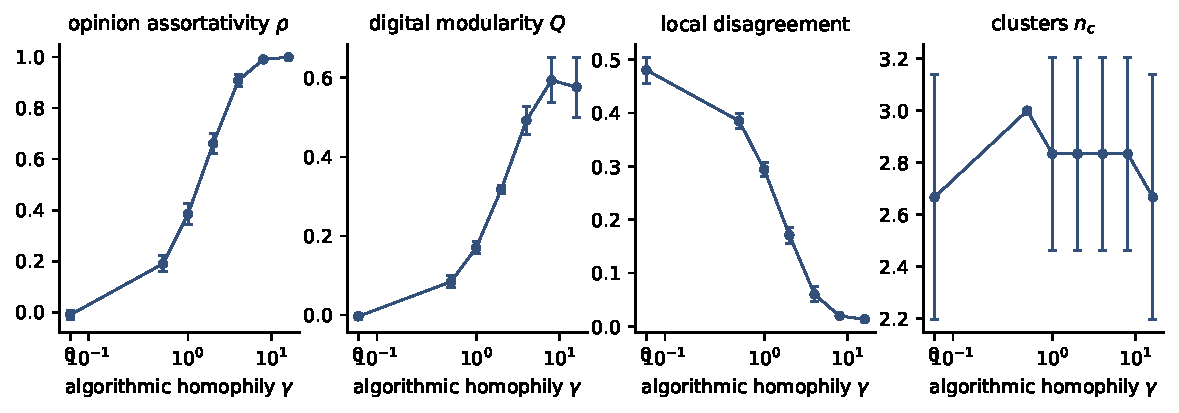
\includegraphics[width=\linewidth]{fig3_adaptive.pdf}
  \caption{Level 3: adaptive digital layer with similarity-driven
  recommendation, $\lambda = 0.5$, $D = 10^{-3}$. From left to right:
  opinion assortativity of the digital graph, modularity with respect to
  opinion clusters, mean local disagreement, and cluster count as functions
  of the algorithmic homophily $\gamma$ (mean $\pm$ s.d.\ over 6 runs).}
  \label{fig:adaptive}
\end{figure}

At Level 3 the platform rewires attention slots with the similarity kernel
$E_{\mathrm{sim}}$. Figure~\ref{fig:adaptive} traces the closing of the
feedback loop opinion $\to$ topology $\to$ exposure $\to$ opinion as
$\gamma$ increases. For $\gamma \approx 0$ the layer behaves like the
neutral platform of Level 2. As $\gamma$ grows, the digital graph
reorganises around the emerging opinion clusters: assortativity climbs
towards one, the modularity of the digital graph with respect to opinion
communities rises, and the average disagreement an agent experiences in its
feed collapses even though the population as a whole remains fragmented.
This is an echo chamber in the precise sense of \citet{baumann2020}: high
global variance, near-zero locally visible disagreement. The mechanism
mirrors the algorithmic-bias model of \citet{sirbu2019}---biased exposure
freezes fragmentation that neutral exposure would have healed---and the
link-recommendation feedback of \citet{santos2021}, transplanted into a
coevolving multiplex \citep{holme2006}. Crucially, these ideological
communities are \emph{spatially delocalised}: their members are scattered
uniformly across the box, so the polarised society shows no geographic
signature whatsoever.

\subsection{Level 4: engagement-maximising platforms and repulsion}
\label{sec:level4}

\begin{figure}[t]
  \centering
  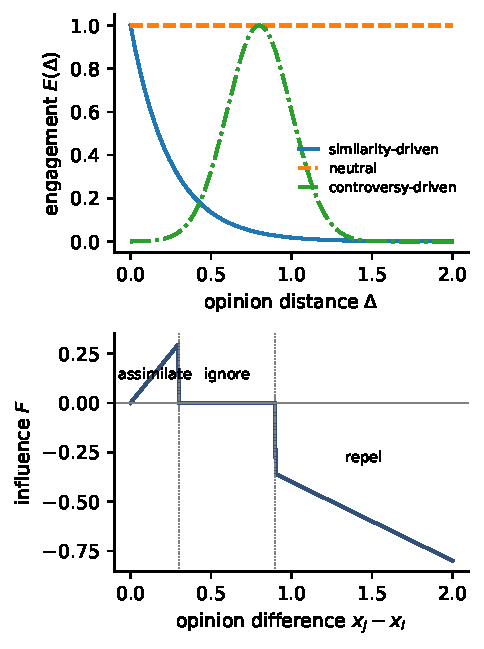
\includegraphics[width=0.8\linewidth]{fig4b_kernels.pdf}
  \caption{Level-4 ingredients. Left: the three engagement kernels of
  Eq.~\eqref{eq:engagement} ($\gamma = 4$, $\delta = 0.8$, $s = 0.2$).
  Right: the assimilation--indifference--repulsion influence function of
  Eq.~\eqref{eq:influence} ($\epsilon_1 = 0.3$, $\epsilon_2 = 0.9$,
  $\eta = 0.4$).}
  \label{fig:kernels}
\end{figure}

\begin{figure}[t]
  \centering
  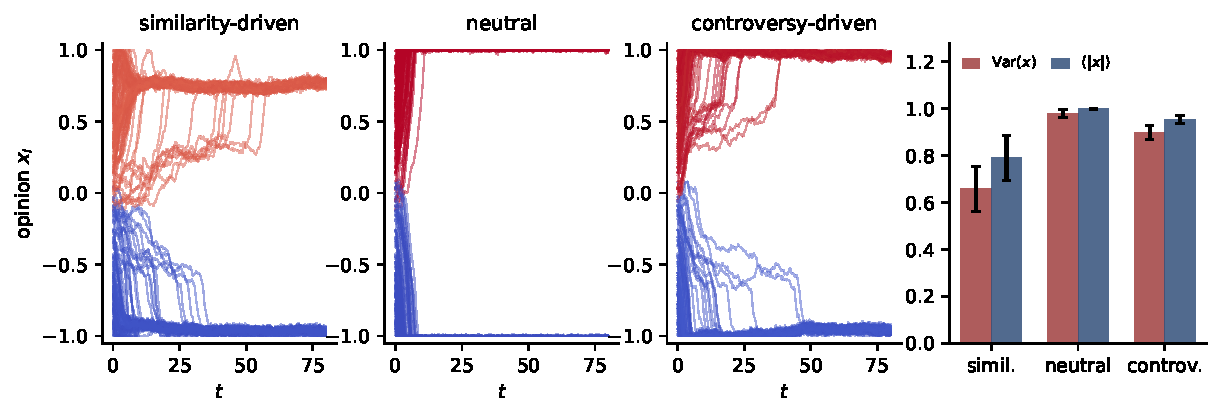
\includegraphics[width=\linewidth]{fig4_engagement.pdf}
  \caption{Level 4: platform designs compared under repulsive influence and
  heavy-tailed influence strengths ($\lambda = 0.6$). Left three panels:
  representative opinion trajectories under similarity-driven, neutral, and
  controversy-driven engagement. Right: polarization $\operatorname{Var}(x)$
  and extremism $\langle |x| \rangle$ (mean $\pm$ s.d.\ over 8 runs).}
  \label{fig:engagement}
\end{figure}

Level 4 activates the repulsive branch of Eq.~\eqref{eq:influence} and
heavy-tailed influence strengths, and compares the three platform designs
of Eq.~\eqref{eq:engagement} (Fig.~\ref{fig:kernels}). The outcome
(Fig.~\ref{fig:engagement}) is unambiguous on one point: once influence can
be repulsive, \emph{every} platform design radicalises the population. All
three designs end with two antagonistic blocs near the boundaries of
opinion space. But the designs differ sharply in degree and speed, and the
ordering is the opposite of what the pure bounded-confidence levels would
suggest. The neutral platform is the most polarizing
($\operatorname{Var}(x) \approx 0.98$, opinions pinned at $\pm 1$ within a
few time units): uncurated exposure samples the full opinion distribution,
which at the start is dominated by pairs beyond the repulsion threshold
$\epsilon_2$, so almost every recommendation triggers mutual repulsion. The
controversy-driven platform is nearly as extreme
($\operatorname{Var}(x) \approx 0.89$) but slower, because its engagement
peak at $\delta = 0.8 < \epsilon_2$ places a substantial fraction of
exposures inside the indifference band where they do nothing. The
similarity-driven platform is the \emph{least} polarizing
($\operatorname{Var}(x) \approx 0.68$): by hiding strongly opposed content
it starves the repulsive channel, and the drift to the extremes---driven by
the residual cross-cutting links that stochastic rewiring keeps
producing---is slow and incomplete. The network signatures also decouple
from the opinion signatures: the neutral platform reaches maximal
polarization with \emph{zero} opinion assortativity ($\rho \approx 0$),
i.e.\ polarization without echo chambers, whereas both curated platforms end
almost perfectly assortative ($\rho \approx 0.9$--$1.0$).

Two lessons follow. First, exposure to disagreement, often proposed as the
remedy for echo chambers, here \emph{is} the engine of radicalisation, as
anticipated by models of partial antagonism \citep{kurmyshev2011,
dearruda2022} and consistent with the empirical evidence that negative
influence is the better-supported micro-mechanism \citep{tang2025}. Second,
whether a given platform design polarises is not a property of the design
alone but of its interaction with the psychology of influence: the neutral
platform is the consensus machine of the assimilation-only world
(Sec.~\ref{sec:level2}) and the radicalisation machine of the repulsive
world, while homophilic curation switches roles in the opposite direction.
In every case the society is simultaneously highly connected (every feed
remains full) and deeply divided: connectivity and polarization are not
opposites.

\subsection{Phase diagram: mobility versus digital attention}
\label{sec:phase}

\begin{figure}[t]
  \centering
  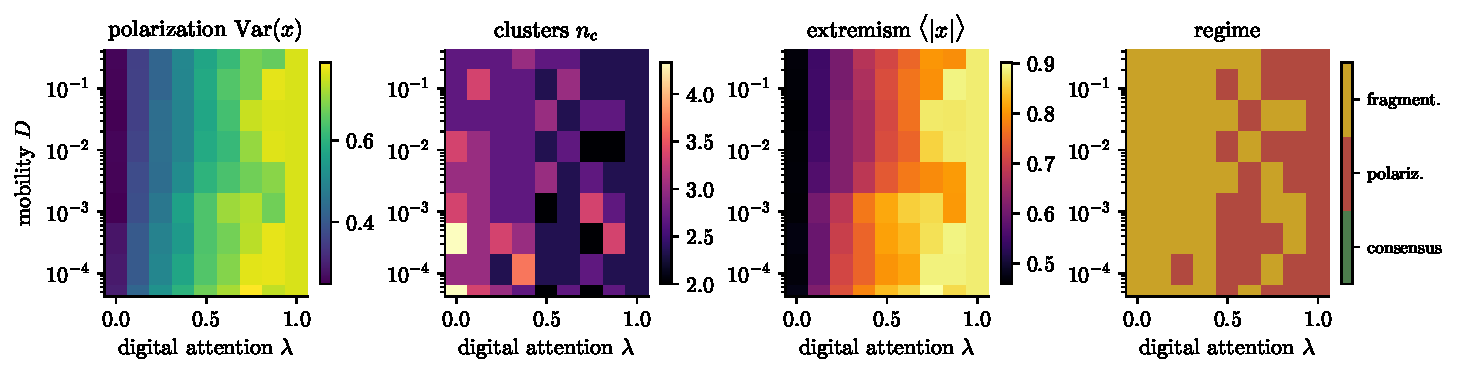
\includegraphics[width=\linewidth]{fig5_phase_diagram.pdf}
  \caption{Phase diagram of the full Level-4 model (similarity-driven
  engagement, repulsion, heavy-tailed influence) in the
  mobility--digital-attention plane. From left to right: polarization
  $\operatorname{Var}(x)$, cluster count $n_c$, extremism
  $\langle|x|\rangle$, and the majority categorical state over 3
  realisations per grid point.}
  \label{fig:phase}
\end{figure}

Figure~\ref{fig:phase} assembles the global picture in the $(D, \lambda)$
plane for the full Level-4 model. The horizontal axis interpolates between
a purely geographical society and a purely platform-mediated one; the
vertical axis spans four decades of mobility. At $\lambda \approx 0$ the
physical layer decides the outcome and the Level-1 crossover is recovered:
frozen local fragmentation at low $D$, the mean-field cluster set at high
$D$. As $\lambda$ grows, the platform captures the attention budget, the
repulsive channel activates through the residual cross-cutting exposure,
and both polarization and extremism rise across \emph{all} mobilities: the
high-$\lambda$ region is a bimodal, radicalised state essentially
independent of $D$. Digital attention thus neutralises the moderating
effect of physical mixing---once the platform curates most of an agent's
exposure, it no longer matters how fast people move. Geography sets the
outcome only for societies whose attention it still owns.

\section{Discussion}
\label{sec:discussion}

\paragraph{Summary.} We built a stochastic adaptive multiplex model coupling
Brownian spatial motion, bounded-confidence social influence, and an
algorithmically curated digital layer under a finite attention budget. The
model reproduces, within one framework, the mobility-controlled
fragmentation crossover of mobile-agent models \citep{alraddadi2024}, the
defragmenting effect of opinion-neutral long-range coupling
\citep{antonopoulos2018}, the echo-chamber feedback of algorithmic homophily
\citep{sirbu2019, santos2021, baumann2020}, and repulsion-driven
radicalisation \citep{kurmyshev2011}, and it locates these outcomes in a
single $(D, \lambda)$ phase diagram.

\paragraph{The geography null result.} The most instructive finding is the
one we did not design for. In the hypothesis motivating this work, strong
digital connectivity would \emph{destroy} geographical opinion structure
while increasing ideological polarization. The simulations show that under
opinion-independent mobility there is no geographical opinion structure to
destroy: locality shapes how many opinions survive but leaves position and
opinion uncorrelated, because disagreeing agents interleave rather than
segregate. The empirically observed geographic clustering of opinion must
then arise from mechanisms outside this model class---homophilic migration,
socially structured mobility, or spatially correlated exogenous influence.
This sharpens the modelling agenda: adding opinion-dependent drift to
Eq.~\eqref{eq:motion} (a Schelling-type term) is the natural Level 5, and
the present model provides the null baseline against which its effect can
be measured cleanly.

\paragraph{No platform design is uniformly safe.} Levels 2--4 give a graded
answer to the public debate on whether platforms polarise, and the answer
is conditional on the micro-psychology of influence. If influence is purely
assimilative (bounded confidence), the neutral platform is actively
beneficial---it supplies the long-range mixing that geography denies to
immobile populations---and the harm comes from similarity curation, which
freezes fragmentation and hides it from its participants behind feeds with
vanishing visible disagreement. If influence has a repulsive component, the
roles invert: uncurated and controversy-seeking exposure manufacture
extremism, and homophilic curation, whatever its epistemic vices, acts as a
buffer against radicalisation. Interventions on recommendation algorithms
that ignore which influence regime the population is in can therefore
backfire in either direction---increasing cross-cutting exposure is
precisely the wrong medicine when negative influence dominates, which is
the mechanism with the stronger empirical support \citep{tang2025}.

\paragraph{Limitations and outlook.} Opinions here are one-dimensional and
confidence bounds static; adaptive-confidence extensions are natural
\citep{li2025}. The attention budget is a fixed split rather than a dynamic
allocation, engagement is a function of opinion distance only, and stubborn
agents were implemented but not systematically explored---sweeping their
number and placement against the platform designs is an obvious next step
\citep{tian2018}. Analytically, the Brownian formulation invites a
continuum (McKean--Vlasov) limit in which the physical term becomes a
nonlocal interaction on a density field and the mixing-time competition can
be made precise; the phase boundaries of Fig.~\ref{fig:phase} are the
natural target of such a calculation \citep{castellano2009, bernardo2024}.

\section*{Reproducibility}

All code, figures, and animation scripts are contained in the accompanying
repository. Each figure is produced by a single script under
\texttt{scripts/}; the model implementation lives in
\texttt{src/socialsim/}; Manim animations of the coupled dynamics are in
\texttt{visualizations/}.

\bibliographystyle{unsrtnat}
\bibliography{references}

\end{document}
